\documentclass[
12pt         % Moar bigger
,twoside     % fogs hates this, but they hate everything
,openright   % fogs hates this too
,versioninfo % useful for drafts
]{mythesis}

% I used these in my thesis.  They're useful.  booktabs makes non-shit
% tables.
\usepackage{graphicx}
\usepackage{amsmath}
\usepackage{booktabs}

\title{your thesis title\\%
  spanning many lines\\so much life}
%
\author{Your Name Goes Here}
%
\month{\textsc{august}} \year{2012}
\previousdegrees{B.Sc., Victoria University of Wellington, 2000\\%
  M.Sc. (Hons), Victoria University of Wellington, 2003}
\degreetitle{Doctor of Philosophy}
\department{Zoology}

\begin{document}

\maketitle

% I worked in different files: input them like so:

\chapter*{Abstract}
\chaptermark{abstract}
\addcontentsline{toc}{chapter}{Abstract}

Many ecological communities show variation from place to place; understanding the causes of this variation is the goal of community ecology. Differences in community composition will be the result of both stochastic and deterministic processes. However, it is difficult to know to what degree, and under which circumstances, deterministic processes will shape community composition. In this thesis I combined observational and experimental approaches to quantify deterministic processes within a particular ecological community -- they phytotelmata of bromeliad plants. In my thesis I describe three studies at different scales of organization: 1) do organisms of different size respond equally to changes in their environment 2) how do predators interact to influence prey survival 3) what mechanisms underly the response of similar species to the same environmental gradient, bromeliad size. 

In Chapter 1, I tested an hypothesis developed from previous observational data - that smaller organisms respond less than larger ones to the same environmental gradient -- different bromeliad species that occur under different forest canopies. I placed identical communities of bacteria, zooplankton and insect communities into bromeliads in different habitats. I found that community composition diverged little for bacteria, more for zooplankton and most of all for macroinvertebrates. In my second chapter, I examined ecological determinism on a smaller scale -- within a single trophic level (macroinvertebrate predators). I found that predators may interfere with each other, reducing predation rates and increasing prey survival. In Chapter 3, I examine macroinvertebrate responses to bromeliad volume. I use a null model to demonstrate that species vary in their response to area more than can be explained by sampling effects alone. Then I discuss a detailed field experiment which showed that for at least one such pair, a difference in abiotic tolerances may be the plausible mechanism. 

Together these results illustrate when, and to what degree, bromeliad communities respond to deterministic factors. All three chapters first demonstrate a pattern, testing it against a suitable null distribution, before attempting to quantify possible mechanisms with a field experiment. This combination of observation and experiment is an approach which can contribute to our understanding of how ecological systems work. 
%%% Local Variables:
%%% TeX-master: "thesis"
%%% TeX-PDF-mode: t
%%% End:

\chapter*{Preface}
\addcontentsline{toc}{chapter}{Preface}

All three chapters in this thesis are original work. The ideas for all chapters were developed by A. A. M. MacDonald and supervisor D. S. Srivastava and were written by A.A.M.M.D. as manuscripts and edited by the co-authors.  Chapter 2 is co-authored with D. S. S., Vinicius Farjalla and Flavia Lima and Alice Campos. V.F. contributed field support and advice on experimental design, while F.L. performed the DGGE analysis of bacterial diversity and A.C counted protists. Chapter 3 is co-authored with D. S. S. and G. Q. Romero, who contributed to the ideas and field support. Chapter 4 is co-authored with D. S. S., who also collected the observational data used in that chapter, while A.A.M.M.D. collected the experimental data.  Field work was completed by A.A.M.M.D. with field assistants Aline Nishi (Chapter 3) and Pedro Trasmonte (Chapter 2 and 4).  All programming and analysis for all chapters was completed by A.A.M.M.D.

%%% Local Variables:
%%% mode: latex
%%% TeX-master: "thesis"
%%% TeX-PDF-mode: t
%%% End:

% This is because FoGS formatting pedandtry is especially accute when
% it comes to tables of contents
\allcontents
% There is currently a problem with spacing somewhere so that Table of
% Contents, List of Tables, and List of Figures have the wrong amount
% of space.  Others are OK though...
\chapter*{Acknowledgements}
\addcontentsline{toc}{chapter}{Acknowledgements}

Acknowledgements are the hardest part of a thesis to write because
they're the only bit most people read.

%%% Local Variables:
%%% TeX-master: "thesis.tex"
%%% TeX-PDF-mode: t
%%% End:

\cleardoublepage
\phantomsection
\addcontentsline{toc}{chapter}{Dedication}
\vspace*{.1\textheight}
\begin{center}
  To Angela
\end{center}

\cleardoublepage
\mainbody

\chapter{Introduction}
\label{chap:introduction}

% Yay inspiriational quotes.
% \begin{quoteshrink}
%   ``At yet higher levels, the species and the community, natural
%   selection obviously must occur. Species evolve to survive in a certain
%   environmental range, and if the environment should suddenly change,
%   some species will become extinct but others will survive.''
%   \hfill\citet{Lewontin-1970-1}, p.~15
% \end{quoteshrink}

\noindent

Observation and experiment are the two fundamental approaches to
understanding ecological systems. In this thesis I use a combination of
observation, null models, and experimental manipulation to understand
what structures aquatic communities in bromeliads. Observational data
are a critical first step in documenting patterns in the natural world.
Null models enhance observational data, as they attempt to represent how
these patterns may have occurred in the absence of a particular
ecological process. As such, when observations exceed the bounds of a
null model, they offer a tantalizing suggestion that the proposed
process might actually be occurring. Experiments can then identify and
isolate which precise process is occurring, and measure its magnitude.
Process is essential to our ability to generalize our results beyond any
one specific system.

But which processes generate patterns of biodiversity in nature that
ecologists seek to explain? Vellend \citep{Vellend2010b} contends that
the myriad of different processes that determine ecological communities
can be grouped into four categories, analogous to the four processes
which underlie evolutionary change: drift, selection, speciation and
dispersal. These processes interact to create the variation we
see among natural communities. Ecological drift is the temporal
variation in the relative abundances of species caused by the sequence
of demographic events within each species. Dispersal is the movement of
organisms or propagules from the regional pool into a local site, which
can introduce new species into a local community. Speciation introduces
new species simultaneously into a community and the regional species
pool, and ecological `selection' determines which particular species
persist in a local patch. Ecological selection refers to the processes
which result in a higher fitness of a given species in a particular
environment relative to all other species present. The similarity
between this process and that of natural selection within a population
is only an analogy, substituting the performance of species for those of
genes. The deterministic nature of ecological selection results in a
nonrandom association between either species and the environment, or
species and each other.

Ecological selection can be predicted by morphological and behavioural
traits of organisms -- i.e., their functional traits. This assumes the
existence of niche-based processes in structuring communities. The niche
is the combination of resource concentrations, and abiotic and biotic
conditions that allow a population to persist. Since the phenotype of
organisms determines the response of the organism to particular
resources or conditions, it stands to reason that the different traits
of organisms then relate to their niche. Traits, however, are
notoriously difficult to measure. Ecologists have therefore proposed
phylogeny as a possible substitute for detailed trait information. This
approach assumes that similarity between species in
ecologically-relevant traits is correlated with the amount of shared
evolutionary history. Phylogeny may go beyond being a (questionable)
substitute for measured traits, and even represent traits which are
difficult to measure \citep{Cadotte2008, Srivastava2012c}. Thus,
nonrandom patterns of either phylogeny or traits are often used as a
means of identifying where niche-based processes are operating. However,
this is not always the case \citep{Mayfield2010}.

The four general categories of ecological processes probably operate in
every system on Earth. However, they cannot be studied everywhere,
usually because of the ``problem of scale'' \citep{Levin1992}: many
systems are too big, or too slow to develop. Therefore, several
empirical ecologists have pursued the study of smaller, simpler systems
(often referred to as ``mesocosms'' or ``microcosms'', to separate them
from larger and more complex systems. This has often been argued to be
the case for natural \citep{Srivastava2004a} and artificial
\citep{W.Fox2007} mesocosms and microcosms. Bromeliads are a key system
because their small size makes them tractable to rapid observation and
manipulative experiment. Bromeliads are home to a wide variety of
animals. These animals interact in a complex food web including
competitors, predators, and even mutualists. Although the habitats are
small, they are neither homogeneous nor very similar to each other --
bromeliads are found in a staggering variety of sites and microhabitats.
Even within a habitat, they span several orders of magnitude in size,
from very small (\textasciitilde{}10ml) to very large (\textgreater{}5L)
plants.

\begin{figure}[htbp]
\centering
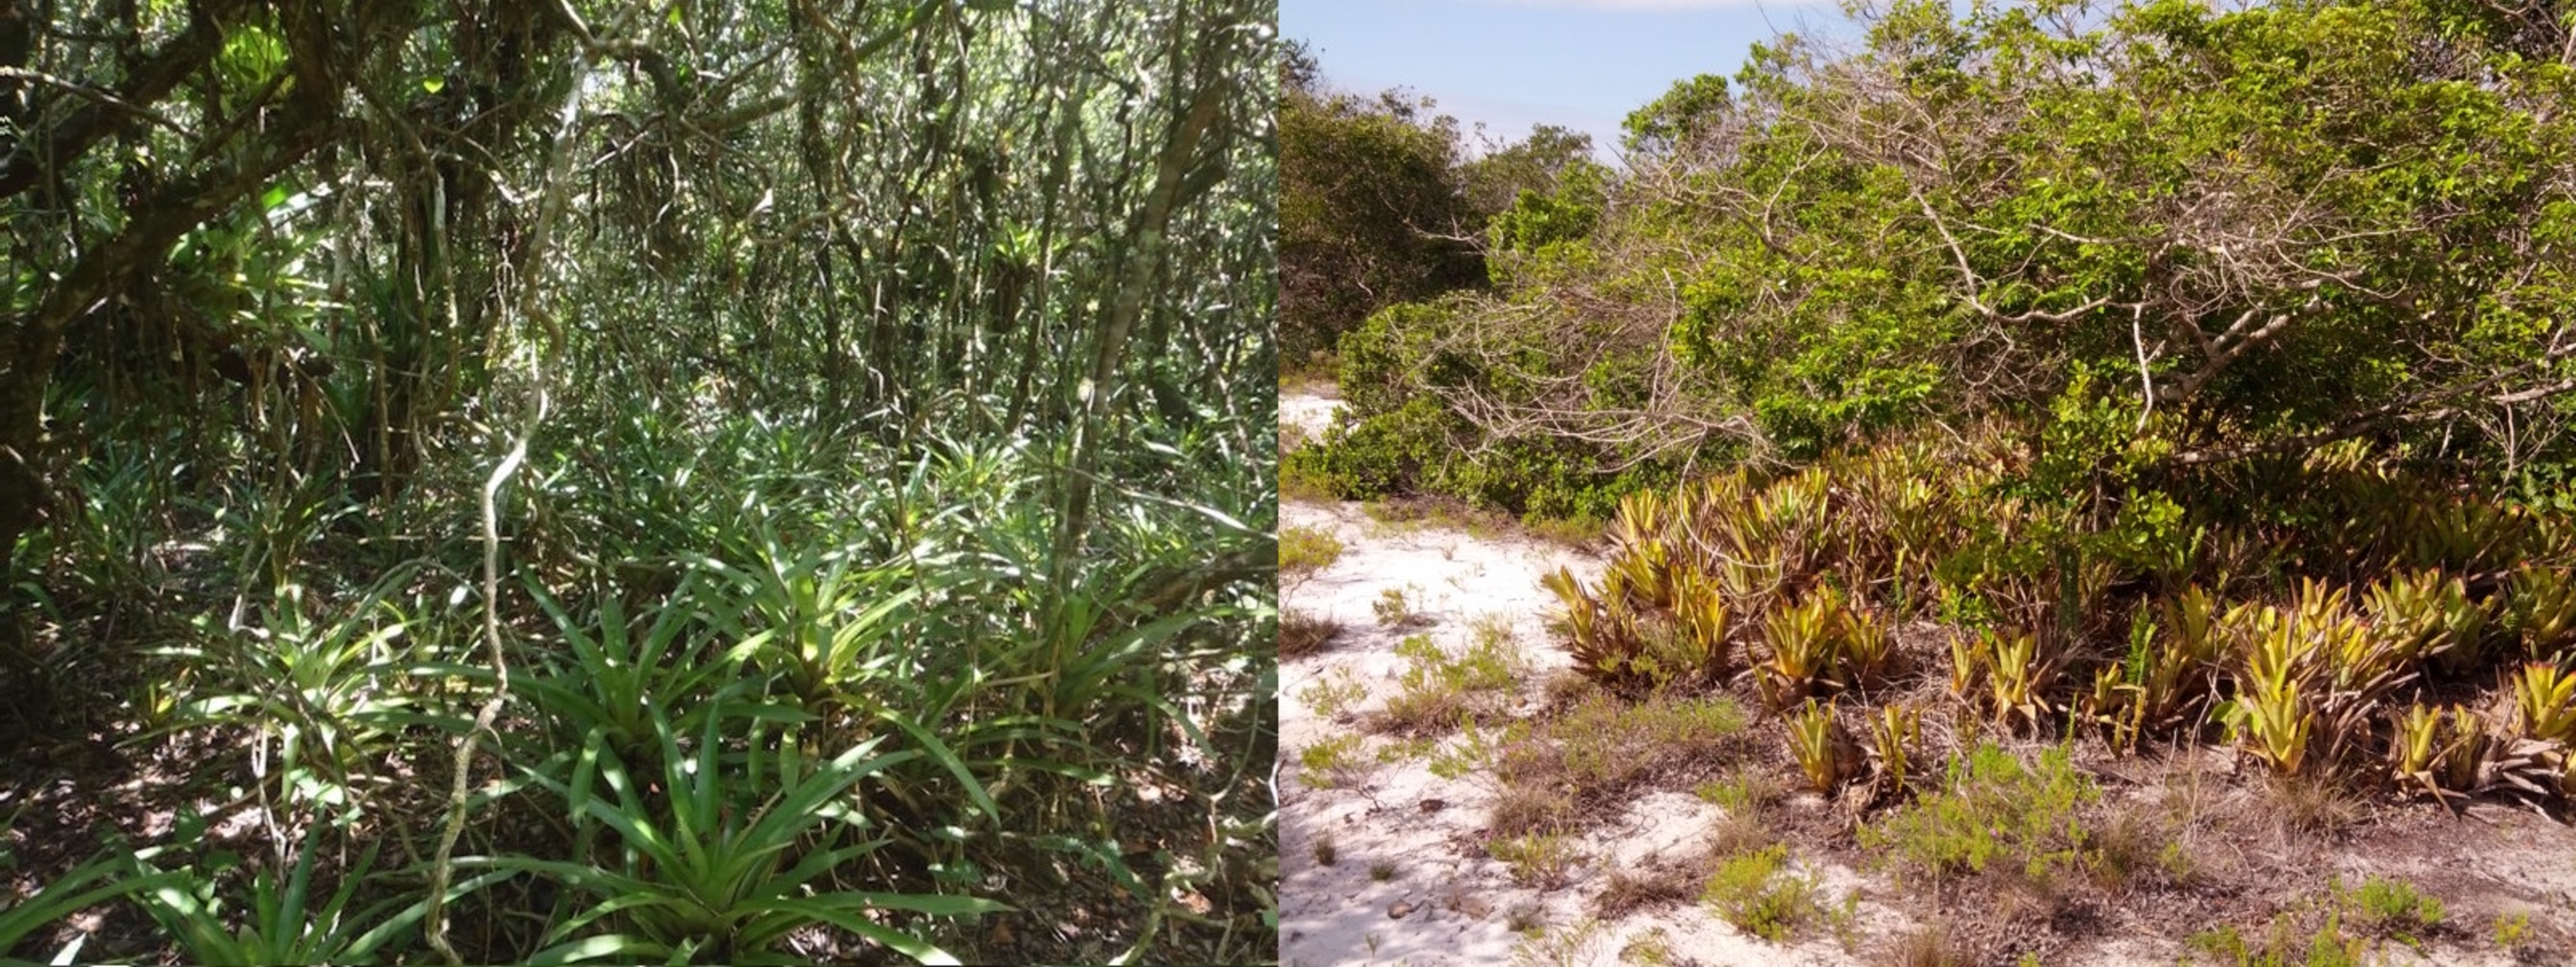
\includegraphics[width=5.5in]{figures/restinga2.pdf}
\caption[Photos of \emph{restinga} vegetation in Brazil]{Photos of \emph{restinga} vegetation in Brazil. \emph{Restingas} are dry, sandy habitats that occur in coastal sites within the Atlantic Rainforest in Brazil. On the left is a forested or ``closed'' restinga which was the location for Chapters 3 and 4. On the right is a more exposed or ``open'' restinga, the site of Chapter 2}
\label{fig:phylo_niche_overlap}
\end{figure}


In this thesis, I take the approach outlined above and apply it to the
tractable model system of bromeliad food webs. I use a combination of
observations and experiments to examine how deterministic and stochastic
processes affect the structure and functioning of these communities. In
each chapter I compare observations against specific null models, to
estimate which processes might be at work. Then, using manipulative
experiments, I test mechanisms suggested by the null models. I examine
two sources of ecological selection: the environment (abiotic) or other
organisms (biotic). Differences in the abiotic environment select for
the presence of different species; this is called habitat filtering.
Habitat filtering has many meanings \citep{Southwood1977, Kraft2015} but
in general refers to a conceptually simple process: among those subset
of species which arrive in a given patch, those who persist must be able
to tolerate both the abiotic and biotic conditions of that patch.

In Chapter 2, I consider the question of which types of organism
(bacteria, zooplankton or macroinvertebrates) show the strongest degree
of habitat filtering. Here, bromeliads offer a rare opportunity to
compare the community structure of these three organisms types -
differing in body size by many orders of magnitude- over the exact same
habitat gradient. In Chapter 3, I first identify the frequent
co-occurrence of predators with one another in bromeliads and overlap in
diets. This suggests the potential for strong predator-predator
interactions, which theoretically can have both antagonistic and
synergistic effects on prey. I use this as an opportunity to determine
how the phylogenetic diversity of predators affects their impact on prey
and ecosystem functions. In Chapter 4, I analyze the differences between
two congeneric species which have very different responses to habitat
size. In this chapter, I also demonstrate that invertebrate species that
live in bromeliads have a strikingly different response to bromeliad
size.

%%% Local Variables:
%%% TeX-master: "thesis"
%%% TeX-PDF-mode: t
%%% End:

\chapter{My incredible discovery}
\label{chap:incredible-discovery}

\section{A section}

The formatting in this style is understated compared with most styles:
no bold serifs and relatively small differences in sizes between types.

\subsection{A subsection}

Subsections are't that much smaller

\subsubsection{A sub subsection}

These are equivalent to the usual paragraph.

%%% Local Variables:
%%% TeX-master: "thesis"
%%% TeX-PDF-mode: t
%%% End:

\chapter{Caveats}
\label{chap:caveats}

\noindent
Put some content in here.

%%% Local Variables:
%%% TeX-master: "thesis"
%%% TeX-PDF-mode: t
%%% End:

\chapter{Conclusion}
\label{chap:conclusions}

\section{Overview of results}\label{overview-of-results}

What creates variation among ecological communities? In this thesis I
have attempted to first demonstrate a number of patterns using
observations, then showed that these patterns are non-trivial with an
appropriate null model, and finally tested those patterns with
controlled field experiments. In Chapter 2, I showed that organisms of
different size respond to different degrees to the same environmental
gradient. Bacterial communities changed very little in response to
habitat differences among bromeliads, while larger organism types
(zooplankton and insects) changed much more. In Chapter 3, I
demonstrated how predator phylogenetic diversity affects ecosystem
function and prey density in a bromeliad system. I showed that unrelated
predators show a nonadditive and negative effect on prey (detritivore)
survival. However, this change in prey density (i.e.~detritivore
density) did not generate an effect on ecosystem function. In Chapter 4,
I showed that related animals tend to be more different in their habitat
size distribution than expected by chance. I demonstrated that, in the
case of two similar chironomid larvae, this difference is caused by
their different responses to the environment: the two congenerics form a
generalist-specialist pair, with otherwise equivalent interactions with
each other and with predators.

Ecologists are confronted by a striking diversity of species
compositions, even within the same community type: not all species are
present everywhere, and even within local scales patches contain only
some of the possible species pool. Where does this variation come from?
It is created by a combination of processes, some of which are purely
numerical or stochastic, others which are deterministic. Vellend
\citep{Vellend2010b} suggests that all the many processes which
ecologists have considered as causes of this variation may be placed
into four categories: ecological selection, drift, speciation and
dispersal. My thesis is an attempt to detect the pattern of ecological
selection (i.e.~the most deterministic of these processes, defined
below) on a particular part of the life cycle of these organisms: the
part spent within the bromeliad mesocosm. However, the results I have
obtained and the patterns I have observed are also connected to the
other three processes. I will rely on Vellend's framework to organise
the remainder of this discussion.

\section{Ecological selection}\label{ecological-selection}

Ecological selection comprises those processes which favour the
occurrence of one species over others. This encompasses such processes
as ``habitat filtering'' (Chapter 2), ``niche partitioning'' (Chapter 4)
and species interactions (Chapter 3). Ecological selection is distinct
from natural selection in that it deals with the persistence of species
through time by demographic processes, not the persistence of genes
through time through inheritance. The environmental conditions of a
local community can determine at least some of the composition of the
species found there. In my thesis I used the naturally patchy mesocosms
found in bromeliads to examine how variation in community composition
arises. Bromeliads are spatially structured -- each individual bromeliad
is a discrete patch of habitat which varies in local environmental
characteristics and colonization histories, and this composite of
abiotic and biotic variables can combine to influence community
composition.

Abiotic variables determining species composition can vary at different
spatial scales. In Chapter 2 and 4 I measured the effect of the abiotic
environment at two scales -- among different bromeliad species in
different habitats (Chapter 2) and among different sizes of the same
bromeliad species (Chapter 4). Both chapters report that associated
environmental differences influence the survival of macroinvertebrate
larvae. Interestingly, this common role of environmental limitation was
found even though the two chapters differ in both the scale of the
gradient and the scale of the taxonomic diversity in the animals
considered. The experiment in Chapter 2 used a very ``steep''
environmental gradient -- different bromeliads in different parts of the
habitat -- and considered responses among all the macroinvertebrates
(across several orders). In contrast, Chapter 4 examined a relatively
subtle environmental gradient (bromeliads of different size, but the same species) and likewise contrasted
two species which were very similar in both taxonomy and morphology
(\emph{Polypedilum}). The study in Chapter 2 (regarding organism size and environmental filtering) presented a more coarse-grained view, reducing the variation
\emph{within} a habitat type to a single factor level (i.e.~bromeliad species/habitat type). Such a study might have
concluded that very similar macroinvertebrates (e.g. \emph{P. marcondesi} and
\emph{P. kaingang}) are able to coexist at that scale. However, Chapter 4
shows that within a single broad ``habitat type'' (i.e.~the same
bromeliad species in the same general habitat), the environmental
differences across different sizes are still important enough to
separate these two species. These two studies illustrate that the
effects of ecological determinism (ecological selection \emph{sensu}
Vellend) caused by the environment is very dependent on the spatial and
taxonomic scale being studied.

Biotic interactions can also impose ecological selection on the
composition of a local community. Negative interactions in particular
can create ecological selection, by limiting local composition to only
those species which can tolerate the interactions. Competition is
frequently considered an important negative interaction within trophic
levels. However, I recovered very little evidence for this process in my
field experiments. In Chapter 4, I did not detect any significant effect
of competition between two functionally similar \emph{Polypedilum}
larvae. There was more evidence for negative interactions within a
trophic level in chapter 3, where I showed that diverse predator
assemblages actually consume \emph{less} prey than monocultures. This is
not resource competition, but rather a kind of predator-predator
interference, possibly caused by the risk of intraguild predation.
Perhaps because of the small, confined nature of bromeliad communities,
such nonconsumptive effects are common between species, and can have
far-reaching consequences on both rates of predation and the functioning
of the entire ecosystem \citep{Atwood2014}. Even if competition is
important among bromeliad invertebrates, coexistence may not be
dependent on partitioning an environmental gradient - for example,
bromeliad size, or different bromeliad species. In fact, divergence
along gradients can sometimes result in competitive exclusion rather
than coexistence \citep{Mayfield2010}. If habitat partitioning of close
relatives is necessary for coexistence, abiotic tolerance traits must be
more labile than traits relating to competition. While this may occur in
allopatric speciation, the opposite pattern is expected in the case of
sympatric speciation. Although the evolutionary biogeography of
bromeliad macroinvertebrates is still unknown, there are examples of
speciation within bromeliads -- e.g.~among Dysticid beetles, whose
association with bromeliads extends back millions of years
\citep{Balke2008} -- and colonization of new species from completely
different habitats -- i.e.~mosquito species switched to bromeliads from
small container habitats \citep{Kitching2001}.

By far the most important negative interaction was predation. Predators
are an important part of the bromeliad community in most parts of the
world, and particularly on Ilha do Cardoso (the field site for Chapters
3 and 4) where they are more numerous, and more diverse, than anywhere else
where formal bromeliad surveys have been conducted (Bromeliad Working
Group, unpub. data). Despite having strong impacts on prey survival,
these predators imposed only weak ecological selection on the
invertebrate community -- consuming prey, but stochastically (i.e.~not
creating variation in species composition: Chapter 4). However,
predators did interact with each other in a negative way, resulting in
less overall predation when predator diversity was high(Chapter 3). Note
that there was no variation in predation effects in Chapter 2, since all
bromeliads contained homogeneous communities (each containing at least
one predator). However, because predators may respond differently than
their prey to the same environmental gradient -- e.g., via changes in
their metabolic rates at higher temperatures -- some of the
environmental effect we observed might have been in part the effect of
predation. This would be analogous to the previously-shown indirect
effects of drought on bromeliad insects via loss of predators
\citep{Amundrud2015}. These results (from all three chapters) suggest that
predators are able to have profound effects on bromeliad communities
once animals have colonized.

\subsection{Taxonomy}\label{taxonomy}

Biotic and abiotic variables only create deterministic selection on
species assemblages when species vary in traits that determine their
response. However, trait data are often lacking, as measurements of
species and individuals are rare. Often, ecologists use patterns of
phylogenetic diversity as a proxy for traits. In this framework, closely
related species are assumed to have similar resource acquisition traits,
and therefore are likely to competitively exclude each other. However,
close relatives might also be very similar in their environmental
tolerance traits and therefore may be likely to co-occur as they respond
in the same way to the same environmental gradient. The bromeliad fauna
of Cardoso lacks a good phylogeny, and therefore I have used taxonomic
categories as a loose guide. This requires the assumption that our
taxonomic categories are good representations of phylogenetic
relationships. Such an assumption may be problematic. The invertebrate
taxa found in bromeliads differ in divergence times by more than 200
million years, so branch lengths within a particular taxonomic level may
be very different. In Chapter 3, we tried to deal with this by using
published estimates for the dates of important nodes in the phylogeny of
predaceous taxa. Incomplete taxonomy poses a second problem: some of our
taxa are identified only to morphospecies, meaning that there may be
more congeneric pairs in this community than we considered. This would
bias our results if we have identified only the most morphologically
distinct subset of congenerics, missing cryptic congenerics which have
been argued to interact more neutrally \citep{Siepielski2010}. On the
other hand, if our selection of congenerics was unbiased, then future
identification of congenerics would only strengthen the power of our
analysis in Chapter 4. More generally, phylogenetic community ecology
assumes that species exclude each other through competition
\citep{Narwani2015}. However, competitive exclusion may be more rare than
ecologists assume, either because inter- and intra-specific competition
are similar \citep{Hubbell1997}, or because strong top-down effects
preclude resource limitation of intermediate trophic levels
\citep{Holt2004}. Therefore, we caution against inferring competition as
the driver of the pattern without evidence of prior competition
\citep{CahillJr.2008}.

\section{Other ecological processes}\label{other-processes}

In all chapters of this thesis, I have tried to measure deterministic
processes. However, there are three other processes which can create
variation in community composition: dispersal, speciation, and drift.
While none of these processes are directly measured in my thesis, they
are all controlled for, or otherwise inform subsequent analysis. More
importantly, as the other three processes create variation in natural
communities, they are critical future areas of study. Below, I briefly
summarize how my methods control for these effects, and also how my
results suggest hypotheses for how they may act in this system.

\subsection{Dispersal}\label{dispersal}

While the abiotic and biotic environments can determine survival of
organisms once they are found in bromeliads, the composition of these
communities is also determined by which animals arrive in the first
place. Dispersal can be either active or passive. In bromeliads, passive
dispersal is usually the action of vectors, such as birds or frogs,
which move from plant to plant. Active dispersal usually takes the form
of a female insect laying eggs in a nonrandom way. Females may select
bromeliads based on their presumed habitat quality for their offspring.
I did not measure female oviposition behaviour directly, but rather the
conditions for larval survival. However, since oviposition behaviour may
be an adaptation to optimize larval performance, the results of these
experiments suggest future hypotheses about how female insects select
oviposition sites.

If female choices are adaptations to maximize larval survival, they may
avoid habitats where their larvae face predation or unsuitable
environments. For example, female insects of many species will avoid
ovipositing eggs into bromeliads with predators inside them
\citep{Hammill2015} or above them \citep{Romero2010}. These
non-consumptive effects can be equal in magnitude to the effects of
predation itself. In a series of feeding trials (Chapter 3), I found
that damselflies consumed more individuals and more species than other
predator taxa. This strong effect of damselfly predation corroborates
previous results from multiple sites \citep{Petermann2015a} and helps explain why
adults avoid ovipositing in bromeliads with damselflies. However, the
results of Chapter 3 suggest a new question. Chapter 3 showed that
damselflies lower their feeding rate when in the presence of other
predators. If so, then this suggests that the identity of the
predator(s) in bromeliads is important for determining the expected
amount of predation, and therefore may influence oviposition decisions
by adults. For example, avoidance of damselflies might be lessened by
the presence of a leech or tabanid. Predator colonization may also be
directly affected: the female damselflies may themselves avoid other
predators. This raises the tantalizing prospect of a
behaviourally-mediated trophic cascade, where fear drives multiple
interactions between trophic levels. Understanding which colonizing
species are important, and the relative importance of colonization
vs.~within-bromeliad predation, will require more detailed field
experiments.

\subsection{Speciation}\label{speciation}

While evolutionary history (as approximated by phylogeny and taxonomy)
may correlate with existing trait variation that is important in
communities, where do these traits come from in the first place?
Speciation introduces new species, which might have different traits
than those already existing in communities. Some organisms found in
bromeliads have close relatives that live in other habitats
(e.g.~caddisflies), while other organisms belong to whole clades of
bromeliad specialists, which speciated after adapting to bromeliads
(e.g. \emph{Mecistogaster} spp. damselflies). Integrating local ecology
with patterns of speciation -- or, similarly, asking how historical
contingency shapes contemporary responses -- has been suggested as an
important future direction in community phylogenetics.
Gerhold et al. \citet{Gerhold2015} call these approaches
``phylogenetic-pattern-as-response'' vs
``phylogenetic-pattern-as-cause''. Understanding the historical
phylogeography of bromeliads would place the results from studies of
species interactions (such as Chapter 3 and 4) into context, allowing us
to relate, for example, interaction strength to the time of association
of two species. In order to fully exploit this advantage of bromeliads,
we would first need a more complete taxonomy and a better phylogeny of
the identified species.

\subsection{Drift}\label{drift}

Drift is the most difficult ecological process to measure, but might be
especially important in small, fragmented habitats like bromeliads.
Drift is caused by the random sequence of demographic events in the life
cycle of organisms, including death, reproduction and dispersal. Drift
therefore generates variation in bromeliad communities from the moment
propagules arrive in bromeliads. Even when dispersal is active, the
number of eggs a female oviposits in a bromeliad may vary among species
and bromeliads. Chironomids, for example, can produce between 80 and 200
eggs \citep{}. We have little information about demographic
rates after oviposition, although studies like that described in Chapter
4 can help us to measure growth and emergence rates. However such
demographic studies are difficult to do for the many species in a
multispecies community. One option for quantifying the role of drift in
multispecies communities is to instead compare compositional change in
identical communities over time \citep{Vellend2010b}. The importance of
drift may also vary across the range of bromeliaceae (across the
Neotropics). The null simulations I performed in this research
(e.g.~Chapter 4) highlight that the patterns we detect are the
result of two different statistical distributions: first, the distribution bromeliad sizes and second, the relative abundance distribution of
bromeliad-dwelling animals. Across habitats, bromeliad size distributions will vary depending on site characteristics and traits of the
bromeliad species present. Meanwhile, the shape of the relative
abundance distribution of insects also varies across sites. Since drift
is most important for rare species and in small habitat patches, the
shape of these two distributions may be very important in determining
the degree to which drift structures communities.

In summary, in this thesis I demonstrated that both the abiotic and the
biotic environment determine the community composition of invertebrates.
Across habitats, invertebrates are more sensitive to environmental
variation than zooplankton and bacteria. Within a habitat, bromeliads of
different sizes may have different environments, with animals showing
specialist-generalist responses to this habitat axis. Biotic
interactions, especially predation, act within and between trophic
levels to influence community composition and/or abundance. Each chapter
of this thesis has demonstrated a pattern in species distribution
against a null model, then quantified the interactions that might have
caused this pattern. Both approaches are key to describing and
explaining the diversity of community types we see in nature.


\formatbibliography
\bibliographystyle{refstyle}
\bibliography{refs-thesis}

\formatappendices
\chapter{Supplementary Information to \Chapref{incredible-discovery}}

\section{A section heading}

\begin{figure}[htbp]
\centering
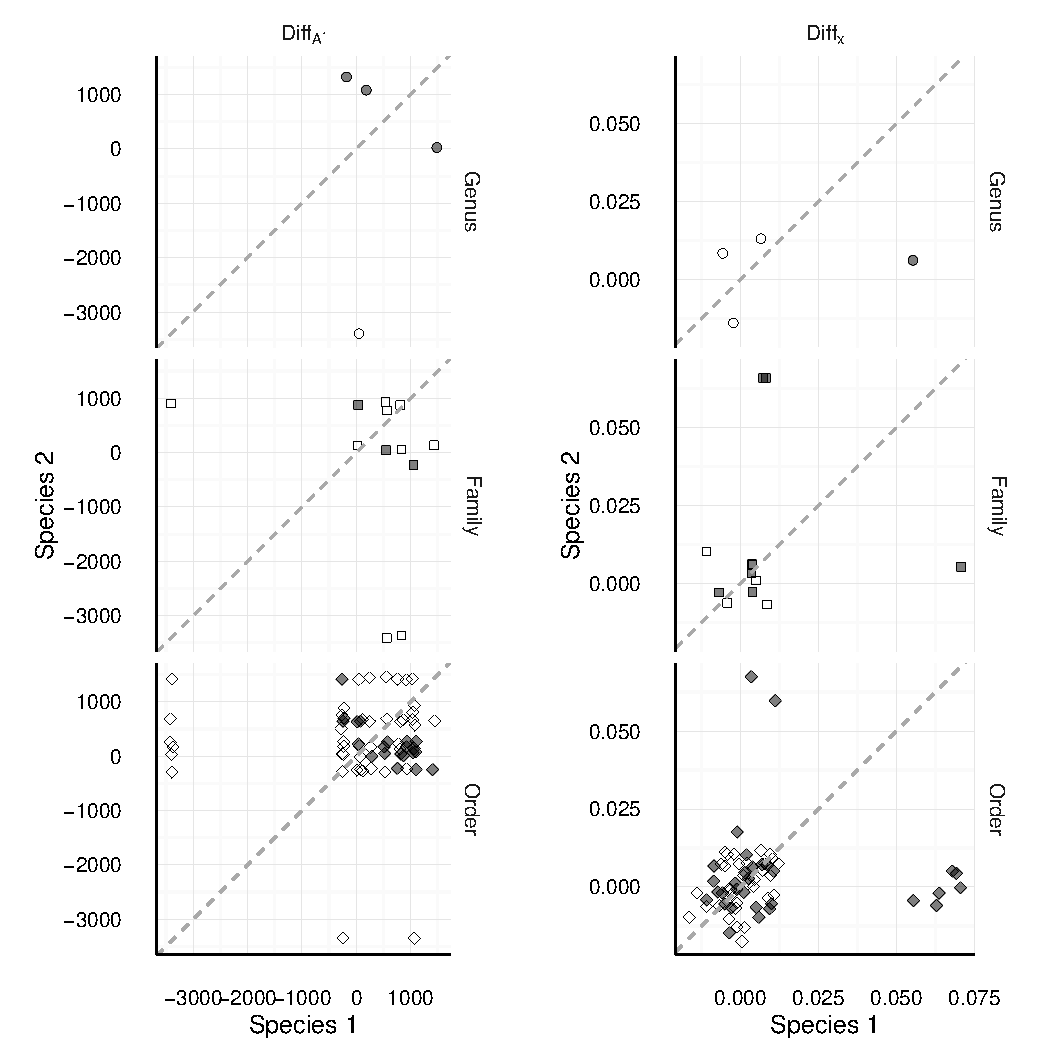
\includegraphics[width=5.5in]{figures/pairwise_astars.pdf}
\caption{Pairwise differences in two measures of size response. Each point represents a
pair of species, divided into species pairs within the same genus (top)
the same family (middle) and order (bottom). The left panel shows
differences in \(A^{*}\) values (units are ml) while the right panel
shows differences in \(x\) (slopes of logistic regression). Species
pairs which are different from a null model are shaded.}
\label{fig:pairwise}
\end{figure}

\begin{figure}[htbp]
\centering
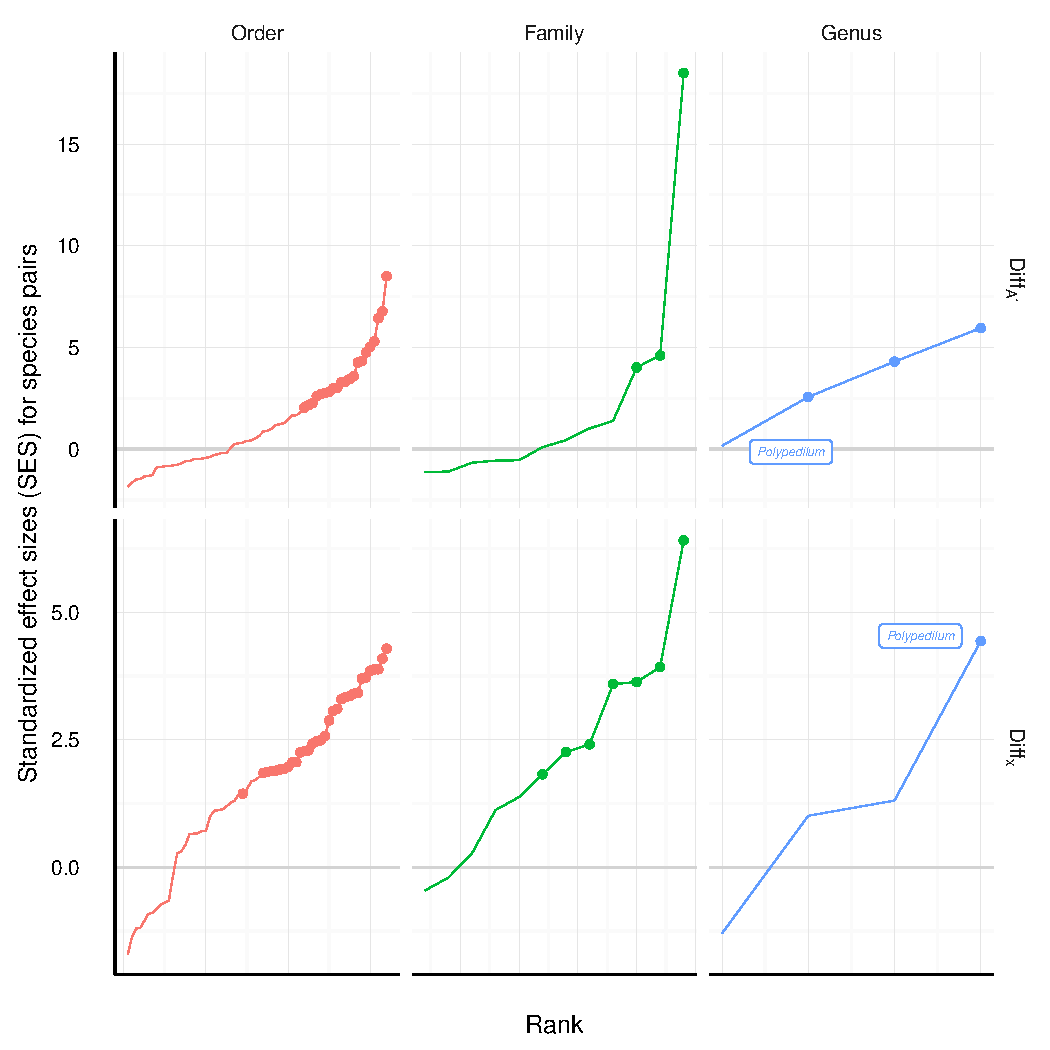
\includegraphics[width=5.5in]{figures/ses_rank.pdf}
\caption{Standardized effect sizes (SES) of pairwise differences
between species for two different measures of patch size response.
These two measures are critical patch size (\(A^{*}\)) and strength of
patch size dependency (\(x\)). Pairwise differences are shown within
each of three taxonomic levels. Significant standardized effect sizes
(randomization p-value \textless{} 0.05) are indicated with points.}
\end{figure}


\end{document}

%%% Local Variables:
%%% TeX-master: t
%%% TeX-PDF-mode: t
%%% End:
